
\documentclass[conference,a4paper]{IEEEtran}

%% depending on your installation, you may wish to adjust the top margin:
\addtolength{\topmargin}{9mm}

%%%%%%
%% Packages:
%% Some useful packages (and compatibility issues with the IEEE format)
%% are pointed out at the very end of this template source file (they are 
%% taken verbatim out of bare_conf.tex by Michael Shell).
%
% *** Do not adjust lengths that control margins, column widths, etc. ***
% *** Do not use packages that alter fonts (such as pslatex).         ***
%
\usepackage[utf8]{inputenc} 
\usepackage[T1]{fontenc}
\usepackage{url}
\usepackage{ifthen}
\usepackage{cite}
\usepackage[cmex10]{amsmath} % Use the [cmex10] option to ensure complicance
                             % with IEEE Xplore (see bare_conf.tex)
\usepackage{graphicx}
\usepackage{subfigure}
\usepackage{hyperref}
\hypersetup{hidelinks}
\usepackage[table]{xcolor}
\usepackage{amssymb}
%% Please note that the amsthm package must not be loaded with
%% IEEEtran.cls because IEEEtran provides its own versions of
%% theorems. Also note that IEEEXplore does not accepts submissions
%% with hyperlinks, i.e., hyperref cannot be used.

\interdisplaylinepenalty=2500 % As explained in bare_conf.tex


%%%%%%
% correct bad hyphenation here
\hyphenation{op-tical net-works semi-conduc-tor}

% ------------------------------------------------------------
\begin{document}
\title{Blueberry Jam: \\Universal Gripper With Computer Vision} 

% %%% Single author, or several authors with same affiliation:
 \author{%
   \IEEEauthorblockN{Junji Hanatani, Jooyeop Kim, Renjie Li, Mike Park}
   \IEEEauthorblockA{ Department of Mechanical Engineering\\
   			Columbia University\\
                     10027 New York, NY\\
                     %Email:  jh3876,jk4109,rl2932,mhp@columbia.com
                     }
 }


\maketitle

%%%%%%%%
%%Abstract%%
%%%%%%%%
\begin{abstract}
  Abstract is \emph{here}.
  
  Describe our mission and general description. Describe our mission and general description. Describe our mission and general description.Describe our mission and general description.Describe our mission and general description.Describe our mission and general description.
  
  Describe our mission and general description.Describe our mission and general description.Describe our mission and general description.Describe our mission and general description.Describe our mission and general description.Describe our mission and general description.
\end{abstract}


\section{Introduction}

The overall goal for this project was to build a functional jamming gripper attachment for the Baxter Robot, as well as incorporating computer vision to enable the robot to autonomously pick and place specified objects into the corresponding hole. The baseline goal for this project was to design and build a working jamming gripper that is able to grasp objects using the camera on the Baxter and lifting the object. This baseline goal acted as proof that our design operated as a functional robotics manipulator. Therefore, if the gripper can grab any object and lift it, we regard it as success. Our main goal is to enable the robot to perform the assembly process. To be specific, through computer vision, the robot must recognize the object, find the hole that matches the surface of the object, and implement the process of accurately placing the object in the hole. Therefore, in addition to grasping, this goal includes recognition with vision sensor and comparing geometry between objects. The motivation for this project is to develop an intelligent robot with versatile grasping capabilities. The jamming gripper can achieve this versatility without complex mechanics and controls like multifingered hands. This technology can be used for manufacturing process (e.g. assembly process). The jamming gripper itself is so soft that it does not damage the object when moving it. Additionally, it is more advantageous in motion planning in terms of shape diversity of grasping, compared to normal gripper. 

\section{System}

\subsection{System Diagram} \label{System Diagram}

\autoref{fig:System Diagram} shows the diagram of our entire system. The jamming gripper with a vacuum pump is attached to the baxter’s left hand. The pump is driven by a motor, which is powered by 12V external power supply, and its driver communicates with the ROS server via arduino (see details in \hyperref[System Diagram]{System Diagram}). The ROS server generates all signals for controlling the baxter’s arm as well as the pump of the jamming gripper. The motion of the baxter arm is basically based on vision feedback. In each time step, the Baxter’s built-in camera captures a 2D image and sends it to the ROS server. In the ROS server, our object detection algorithms identify the pixel positions of the objects in the image and generate feedback signals based on PID method. (See details in section 204,2-5.)

\begin{figure}[h]
\centering
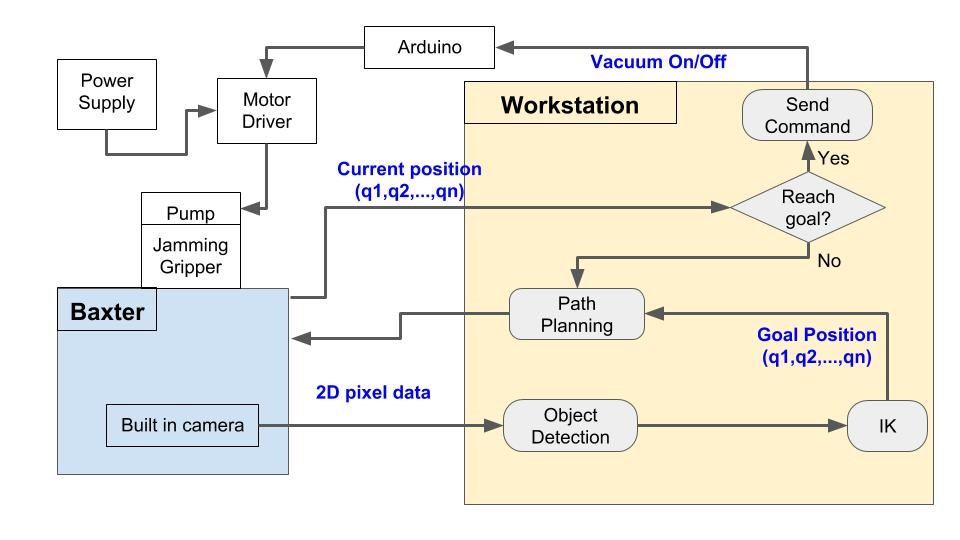
\includegraphics[width=0.5\textwidth]{System_Diagram.jpg}
\caption{System Diagram}
\label{fig:System Diagram}
\end{figure}

\subsection{Differences from PDD}

In our PDD, we suppose to use a RGB-D camera (e.g. Microsoft Kinect, Asus Xtion Pro) mounted on Baxter to identify the rough position of the objects and then move the Baxter arm to the corresponding location. But in our final product, this idea was abandoned due to the software issues. At the very beginning, we believe the port on the back of the Baxter robot will natively support the RGB-D camera. However, it cannot do that. We tried another method: connect the Asus Xtion Pro to the computer and use the computer as a communication bridge between the Baxter and our jamming gripper. Disappointedly, it still cannot work. The RGB-D camera could only work properly (but not stably) on the administrator account in this computer. Because of this (plus we do not have enough time left -- we find ourselves unable to solve this problem one month ago) , we decide to abandon this idea. Instead, we would hardcode the rough position of the objects. This is the only difference from the PDD in our final product. 

\subsection{Hardware Components}

The Jamming gripper works as follows: First, after the gripper arrives at the target object, wait for the balloon to fully enclose the object, and the pump works to suck the air and grasp the object. 
	
Our gripper consists of the following components: balloon, coffee, air pump, tube, motor driver, arduino, case, funnel and filter.

\begin{figure}[h]
\centering
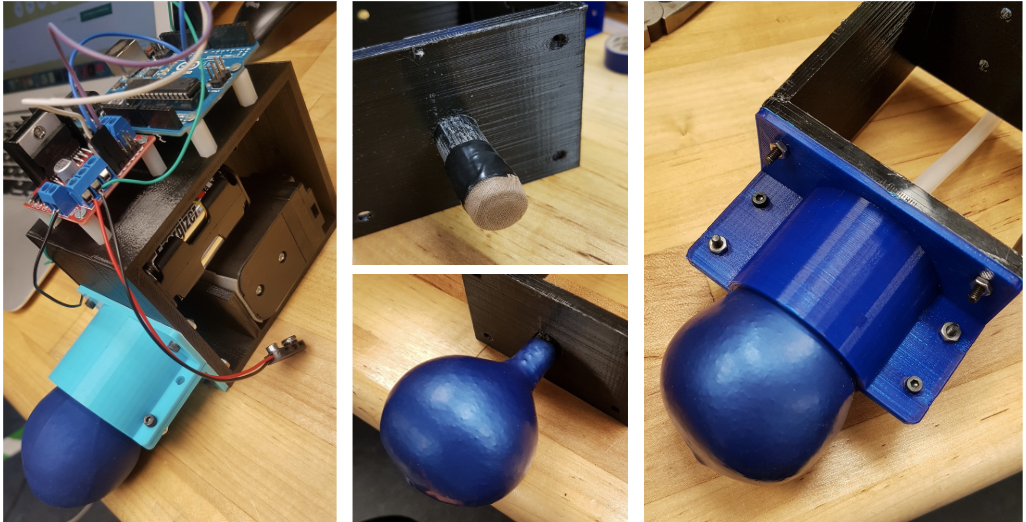
\includegraphics[width=0.5\textwidth]{Hardware_Components.png}
\caption{Hardware Components (from left to right: a,b,c)}
\label{fig:Hardware Components}
\end{figure}

In \autoref{fig:Hardware Components}(a), all the components are shown. The case has space for attaching the air pump and battery, while the Arduino and motor driver are attached on the outer wall of the case with spacers. Also, the case has a stem to attach filter and balloon, and connect the part with tube for air pump in \autoref{fig:Hardware Components}(b). The inner diameter of the stem is designed to match the outer diameter of the tube, and the outer diameter is set so that the balloon has sufficient tension. The balloon is filled with coffee as granular material. In \autoref{fig:Hardware Components}(c), the funnel is attached in a way that two separate parts are assembled, which adds to the usability in assembly.

Arduino board receives the signal from the ROS and operates the motor and controls the motor through the motor driver. The battery serves to power the motor driver to drive the pump, which was later replaced by a power supply for more powerful power.

\subsection{Trial \& Error for Design}

While implementing the gripper performance with baxter, several problems occurred, and the design was modified accordingly as follows.

\begin{figure}[h]
\centering
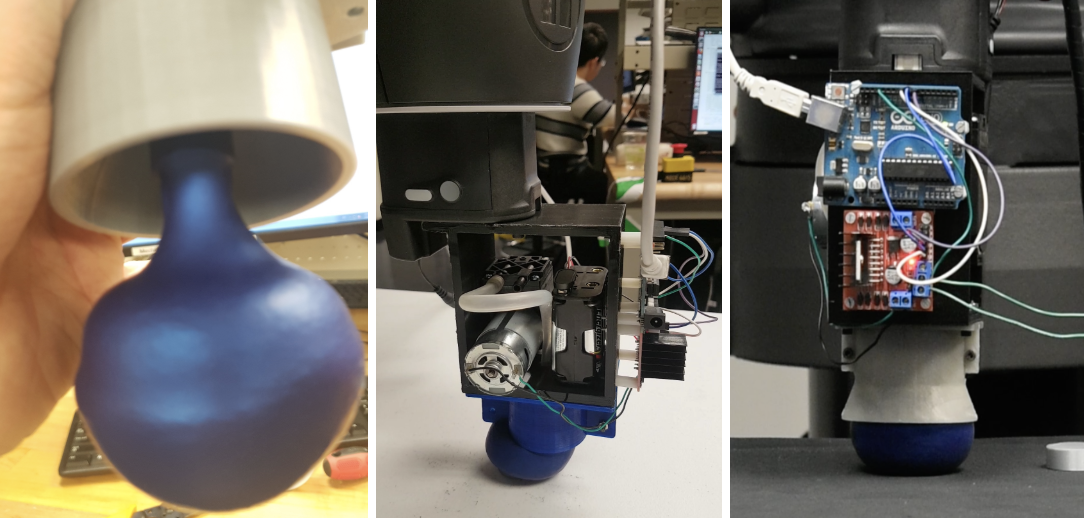
\includegraphics[width=0.5\textwidth]{Trial_Error.png}
\caption{Modification for Gripper Design (from left to right: a,b,c)}
\label{fig:Trial Error}
\end{figure}

\subsubsection{Hanging}
When attaching the balloon to the stem without removing the band of the balloon, the phenomenon occurs as shown in \autoref{fig:Trial Error}(a). This problem was solved by shortening the balloon. 
\subsubsection{Moment}
A moment occurred in the initial design because there was a distance between the point at which the gripper touches the object (ie, the center of the balloon) and the point at which the force of the baxter arm is applied. As a result, in \autoref{fig:Trial Error}(b), the balloon was dragged, which has affected negatively the grasping performance. To solve this problem, the design was modified to reduce the distance. That is, the balloon is positioned at the center of the arm as much as possible.
\subsubsection{Diameter of Funnel}
For the jamming gripper to work properly, there must be enough space for balloons to spread. In previous design, however, the funnel used a minimum diameter to prevent interference with the camera's field of view(because the balloon was moved as close to the camera as possible to eliminate moment). It gave bad influence. Thus, even though there was some visual disturbance, the diameter of the funnel was increased and the better results were obtained.
\subsubsection{Battery Power}
During the experiment, due to the vibration generated by the pump and baxter, a stronger pump force was required. When using alkaline batteries, we could only use 30\% of the pump's power, so we increased the power by connecting an external power supply instead of battery sets.



\subsection{Serial Communication \& Motor Control}

Shown in \autoref{fig:System Diagram}, Arduino Uno is the communication bridge between the motor driver (via Pin 7-9 \& GND in Arduino, and in1-2 \& enA in driver) ,the Ubuntu desktop (via USB Type B cable) and the Baxter. The motor driver that we use is L298N Dual H Bridge Motor Driver, it is powered by 12V power supply. The vacuum pump is connected to the vout port of the motor driver. 

In our Baxter program, every time the Baxter moves to the right position, which is our approaching part (will discuss later), the program will publish an Empty topic named `pump\_on' and publish another `pump\_off' after all the grasping tasks are finished. The communication between Arduino and Baxter (ROS) is implemented by a node named Rosserial. Arduino will continuously wait for the message published from ROS. When `pump\_on' is received, the Arduino will set pin 8 as high,  pin 7 as low, (pin 9 is an analog pin that may control the power of the motor by PWM)which may turn on the motor and vice versa.


\subsection{Object Detection}
The goal of our object detection algorithms is to identify the location of objects that have simple shapes such as a square, a triangle, and a circle, in the input image. To achieve that, we implement object detection algorithms as described below:

\begin{figure}[h]
\centering
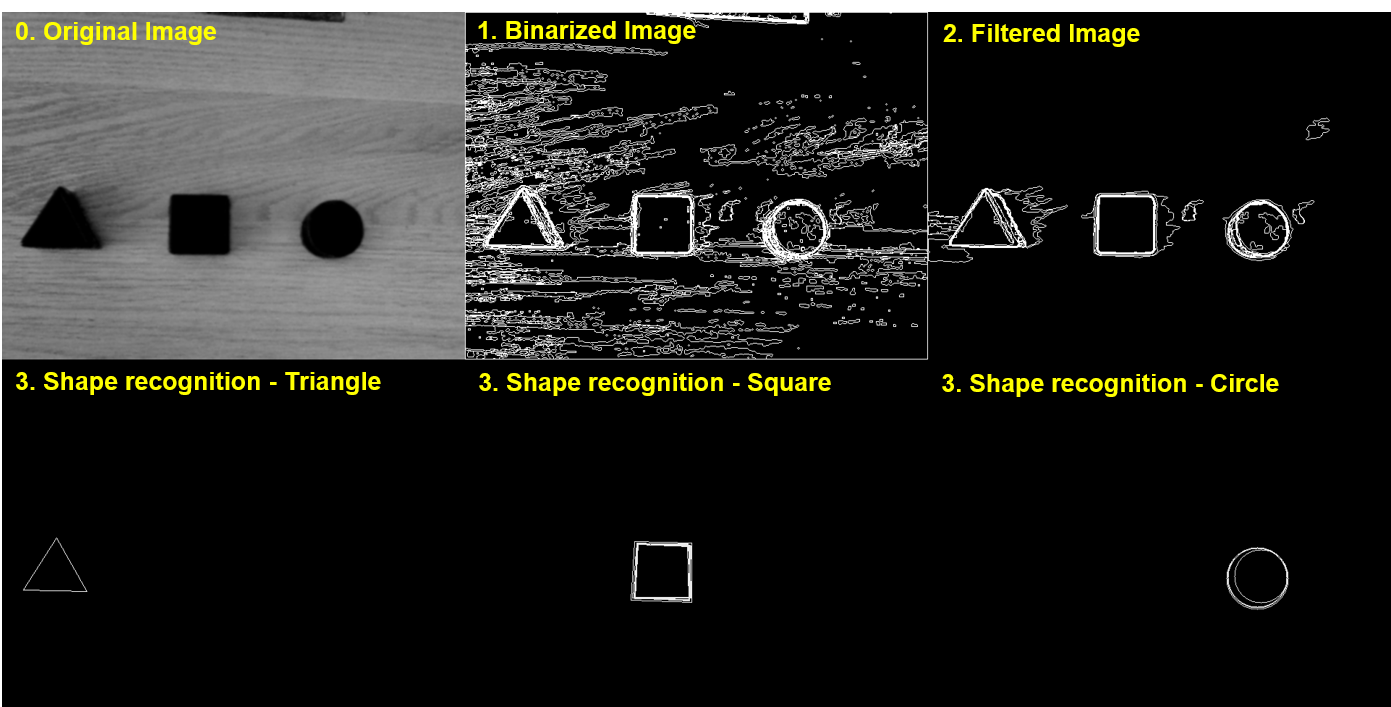
\includegraphics[width=0.5\textwidth]{ObjectDetection.png}
\caption{Object Detection}
\label{fig:Object Detection}
\end{figure}

\subsubsection{Image Binarization}
Split original color image into R,G,B data and binarize each image using Canny edge detector and 5 threshold values. Thus, finally we have 6$\times$3 (R,G,B) = 18 binary images. 
\subsubsection{Object Segmentation}
For each binary image, draw contours and extract objects.
\subsubsection{Filtering(Size\&Aspect Ratio)}
%Pick up the shapes based on the criteria below:
\begin{itemize}
\item Square: Object consists of 4 lines and the angles are approximately 90deg.
\item Triangle: Object consists of 3 lines and the angles are approximately 60deg.
\item Circle: Object area is nearly equal to the area of minimum enclosing circle.
\end{itemize}

\subsubsection{Center Position Calculation}
For triangle and square, we can obtain center positions by simply taking the average over all vertex positions. For the circle, we just use the center of the minimum enclosing circle of the objects (The function is available in the OpenCV library.)

\subsection{Motion Planning}

To achieve our goals, we divide the tasks into several steps and generate the motions for each task in an appropriate manner. These motions are sequentially executed as described below:

\begin{figure}[h]
\centering
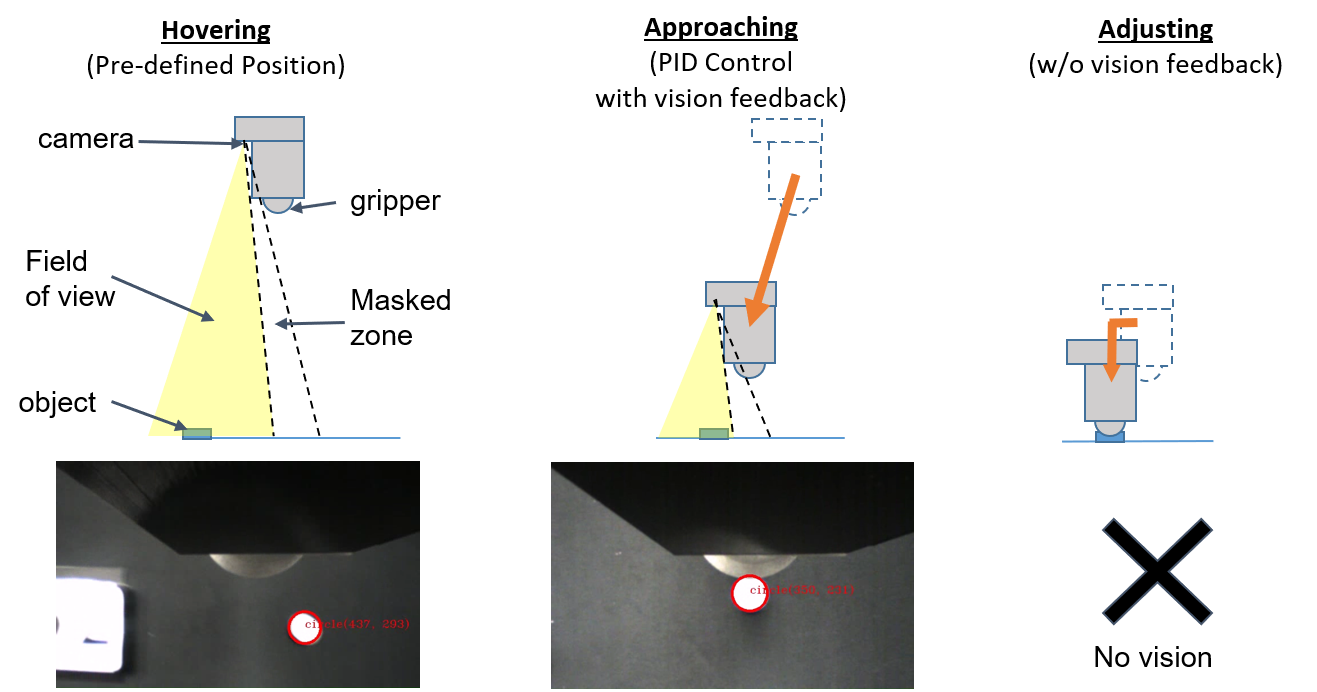
\includegraphics[width=0.5\textwidth]{MotionPlanning.png}
\caption{Motion Planning}
\label{fig:Motion Planning}
\end{figure}

\subsubsection{Hovering} The arm moves to the pre-defined position (roughly above the objects,) and wait in the air.
\subsubsection{Approaching} Once the camera finds the target object, the arm approaches to the object with vision feedback. In our PID controller, the reference value is given as a pixel position and compared with the current pixel position of the object, which is identified by the object detection algorithm in each time step. 
\subsubsection{Adjusting} Even after the approaching step, the gripper cannot reach just above the object. This is because when the gripper approaches closer to the object, the target object disappears from the image due to overlapping with the jamming gripper itself, and thus the vision feedback no longer functions. Therefore, in this step, the gripper moves a pre-defined distance to reach just above the object.  
\subsubsection{Grasping} push the object to the table and send an activation signal to arduino to turn on the jamming gripper, then wait 7 seconds to make sure that the air is sufficiently evacuated from the gripper.
\subsubsection{Retracting} Move back to the hovering position described above (Step.1)
Repeat the same motion for the corresponding hole.

For the ?Adjusting? step, we repeated trials to calibrate the amount of motion. However, due to the baxter's motion error, we found that the resulting position is slightly different each time. We will discuss this motion error in the section 3-3.



\section{Experiment}

\subsection{Description}
In the experiment, the robot recognizes the shape matching the command and picks up the object and carries it to the corresponding hole.
 
The experimental environment is as follows: Place a triangular, square, or circular object in a row on a desk and a frame with each type of hole next to it. To solve the shadow problem, the desk was covered with a black cloth, and the color of each object was made in a color contrasting with black.

\subsection{Success Criteria}
\begin{itemize}
\item The jamming gripper will succeed in grasping 3/3 objects at a success rate of at least 75\% each.
\item The jamming gripper will succeed in identifying the shape of 2/3 objects and placing them into the corresponding holes at a success rate of 75\% each.
\end{itemize}

Here, grasping success indicates when the robot lifts the object vertically. Detecting success is when the robot places the gripper on an object that matches the command. Transporting success indicates when the robot moved objects into the corresponding holes. 


\subsection{Result}

The experiment was implemented 25 times for all objects:

    \begin{table}[h]
        \centering
        \scalebox{0.8}{
        \begin{tabular}{|c|c|c|c|c|c|c|c|c|c|}
            \cline{1-10} 
             Action & \multicolumn{3}{c|}{Detect} & \multicolumn{3}{c|}{Grasp} & \multicolumn{3}{c|}{Transport}\\
            \cline{1-10}
             Object & $\triangle$ & $\square$ & $\bigcirc$ & $\triangle$ & $\square$ & $\bigcirc$ & $\triangle$ & $\square$ & $\bigcirc$ \\
            \hline
            Success & \cellcolor{green!25}100\% & \cellcolor{green!25}100\% & \cellcolor{green!25}100\% & \cellcolor{green!25}88\% & \cellcolor{yellow!25}72\% & \cellcolor{green!25}92\% & \cellcolor{green!25}84\% & \cellcolor{yellow!25}52\% & \cellcolor{green!25}88\% \\
            \hline
            PDD & 75\% & 75\% & 75\% & 75\% & 75\% & 75\% & 75\% & 75\% & 75\%  \\
            \hline
        \end{tabular}}
       % \caption{Mul}
        %\label{multiprogram}
    \end{table}

As a result, we successfully performed except the grasping and transporting object for the square.

\subsection{Result Analysis}

\begin{figure}[h]
\centering
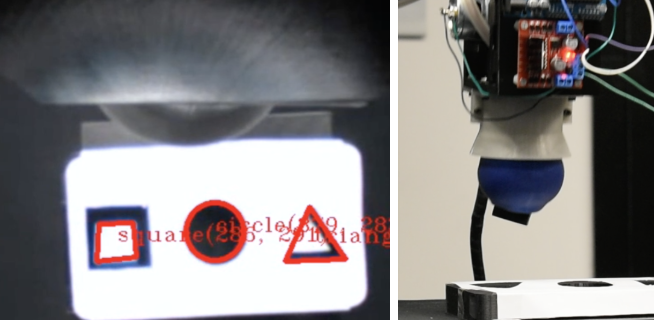
\includegraphics[width=0.5\textwidth]{Analysis.png}
\caption{Result Analysis (from left to right: a,b)}
\label{fig:Analysis}
\end{figure}

In the experimental results, only square case did not meet the criteria. This may be due to the failure of motion planning derived from incorrect pose estimation. As shown in \autoref{fig:Analysis}(a), the detection of square was not necessarily a square, but a {\it distorted} rectangle. In that case, it was difficult to estimate the position of object accurately, and it was hard to locate the gripper at the center of the object. On the other hand, almost perfect recognition was achieved for the circle, showing a success rate close to 90\%.


\subsection{Unexpected Problems}

\subsubsection{Stickiness}
Unexpectedly, due to the stickiness of the balloon, the object was still stuck from the gripper even though the pump was turned off.

 {\bf Possible Solution:} To avoid sticking, the jamming gripper needs to have a blower pump as well as a suction pump. When the gripper release the object, a blower pump helps the object detach from the sticky rubber by extending the gripper surface.
\subsubsection{Inaccuracy of Baxter}
Because of baxter's inaccuracies, the parameters were modified every time and different results were obtained with the same parameters.

 {\bf Possible Solution:} As mentioned in the section 2.4, Baxter's motion error in the "Adjusting" step cannot be corrected by vision feedback, because the target object disappears from the image. This motion error considered to be mitigated when the baxter approaches closer to the object with vision feedback, i.e., the amount of the motion in the 
"adjusting" step is reduced. Thus, the success rate can be improved by two approaches below:
 \begin{itemize} 
\item Re-design more compact outer case for the gripper than the current design so that the masked zone in the image is reduced.
\item Develop another algorithms for object detection that can detect the object even if the part of the object is missing due to overlapping.
\end{itemize}
\section{Conclusion}

\subsection{Recap}

\subsection{Future Works}


\section*{Acknowledgment}

Thank you guys.


%%%%%%
%% To balance the columns at the last page of the paper use this
%% command:
%%
%\enlargethispage{-1.2cm} 
%%
%% If the balancing should occur in the middle of the references, use
%% the following trigger:
%%

%\IEEEtriggeratref{3}

%%
%% which triggers a \newpage (i.e., new column) just before the given
%% reference number. Note that you need to adapt this if you modify
%% the paper.  The "triggered" command can be changed if desired:
%%
%\IEEEtriggercmd{\enlargethispage{-20cm}}
%%
%%%%%%


%%%%%%
%% References:
%% We recommend the usage of BibTeX:
%%
%\bibliographystyle{IEEEtran}
%\bibliography{definitions,bibliofile}
%%
%% where we here have assume the existence of the files
%% definitions.bib and bibliofile.bib.
%% BibTeX documentation can be obtained at:
%% http://www.ctan.org/tex-archive/biblio/bibtex/contrib/doc/
%%%%%%


%% Or you use manual references (pay attention to consistency and the
%% formatting style!):
%\begin{thebibliography}{9}
%
%\bibitem{Laport:LaTeX}
%L.~Lamport,
%  \emph{\LaTeX: A Document Preparation System,} 
%  Addison-Wesley, Reading, Massachusetts, USA, 2nd~ed., 1994. 
%
%\bibitem{GMS:LaTeXComp}
%F.~Mittelbach, M,~Goossens, J.~Braams, D.~Carlisle, and
%C.~Rowley, \emph{The {\LaTeX} Companion,} Addison-Wesley,
%Reading, Massachusetts, USA, 2nd~ed., 2004.
%
%\bibitem{oetiker_latex}
%T.~Oetiker, H.~Partl, I.~Hyna, and E.~Schlegl, \emph{The Not So Short
%  Introduction to {\LaTeX2e}}, version 5.06, Jun.~20, 2016. [Online].
%  Available: \url{https://tobi.oetiker.ch/lshort/}
%
%\bibitem{typesetmoser}
%S.~M. Moser, \emph{How to Typeset Equations in {\LaTeX}}, version 4.6,
%  Sep. 29, 2017. [Online]. Available:
%  \url{http://moser-isi.ethz.ch/manuals.html#eqlatex}
%
%\bibitem{IEEE:pdfsettings}
%IEEE, \emph{Preparing Conference Content for the IEEE Xplore Digital
%  Library.} [Online]. Available:
%  \url{http://www.ieee.org/conferences_events/conferences/organizers/pubs/preparing_content.html}
%
%\bibitem{IEEE:AuthorToolbox}
%IEEE, \emph{Author Digital Toolbox.} [Online.] Available:
%  \url{http://www.ieee.org/publications_standards/publications/authors/authors_journals.html}
%
%\end{thebibliography}


\end{document}



